\documentclass[11pt,a4paper]{article}
\usepackage[utf8]{inputenc}
\usepackage[T1]{fontenc}
\usepackage{amsfonts}
\usepackage[french]{babel}
\frenchbsetup{StandardLists=true} % à inclure si on utilise \usepackage[francais]{babel}
\usepackage{enumitem}
\usepackage{amssymb}
\usepackage{amsmath}
\usepackage[left=2cm,right=2cm,top=2cm,bottom=2cm]{geometry}
\usepackage{multirow}
\usepackage[dvipsnames]{xcolor}

\usepackage[T1]{fontenc}
\usepackage{fouriernc}
\usepackage{graphicx}

\usepackage{setspace}
\singlespacing

\usepackage{pstricks}
\usepackage{xkeyval}
\usepackage{pst-labo}


\usepackage{multicol}
\usepackage{caption}
\usepackage{fancyhdr}
\pagestyle{fancy}
\renewcommand\headrulewidth{1pt}
\fancyhead[L]{Lycée Denis Diderot }
\fancyhead[R]{Classe de 1 Bac Pro }
\setcounter{page}{1}\fancyfoot[C]{page \thepage}
\fancyfoot[R]{Année 2024-2025}
\fancyfoot[L]{Chapitre 4 - Pression et forces pressantes}
\usepackage{multirow,tabularx,booktabs}
\newcommand{\cadreblanc}[1]{%
\medskip\framebox[\linewidth][c]{%
\rule{0mm}{#1mm}}\par
\medskip}

\usepackage{awesomebox}
\setlength{\aweboxvskip}{0mm}
\usepackage{pifont}
\usepackage{chemmacros}
\chemsetup{modules=all}
\setlength{\columnseprule}{.25mm}

\renewcommand{\arraystretch}{2}
\newcommand*\acocher{\quitvmode{\fboxsep0pt \fboxrule0.8pt \fbox{\vrule height1.8ex depth.1ex width0pt \vrule height0pt depth0pt width1.9ex }}}

\newcommand{\code}{\awesomebox[black]{2pt}{

\includegraphics[scale=0.15]{../Chapitre 1 - Energie et puissance électrique/images/frame.png}
}{black}}

\newcommand{\moteur}{\awesomebox[black]{2pt}{

\includegraphics[scale=1]{images/moteur.jpg} 
}{black}}

\newcommand{\defconclusion}{\awesomebox[black]{2pt}{\rotatebox{90}{\Large{\textbf{Conclusion}}}}{black}}

\frenchbsetup{StandardLists=true}



\begin{document}


\begin{center}
 \LARGE{Activité 1 - Expérience pour caractériser la pression atmosphérique }
\end{center}



\normalsize

\hrule\
\\[0,2cm]

\begin{center}
    \textbf{L'air atmosphérique est attiré par la Terre et tombe comme n’importe quel objet.
Il exerce donc une force pressante sur tous les corps à la surface de la Terre et par là même exerce une pression : la
pression atmosphérique.}
\end{center}

\vfill 

\fbox{1. Hémisphères de Magdebourg}

%\noindent%
\begin{minipage}{.75\textwidth}%
 
Deux hémisphères creux d'un peu plus de cinquante centimètres de diamètre furent assemblés pour former une sphère ; un des hémisphères était muni d'un tube fermé par une valve. Le tube était relié à une pompe à vide inventée par Otto von Guericke. L'air contenu dans la sphère put être pompé, créant ainsi un certain vide. Le premier vide artificiel avait été produit.  La différence de pression entre l'extérieur et l'intérieur des hémisphères les maintenait fermement ensemble en les comprimant. 
 
\end{minipage}%
\hfill
\begin{minipage}{.20\textwidth}%
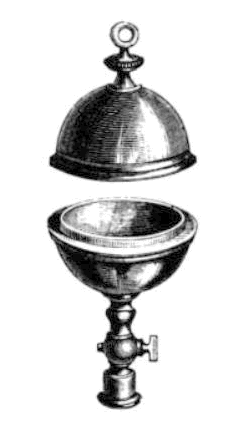
\includegraphics[width=\textwidth]{images/Magdeburg_hemispheres_small.png}
\end{minipage}%

%\vfill

\fbox{2. La cloche à vide}



\cadreblanc{50}

\vfill

\fbox{3. Expérience : mise en évidence de la pression atmosphérique}

\cadreblanc{50}

\vfill 

\newpage

\hrule


\begin{center}
 \LARGE{Activité 2 - Pourquoi certains musés interdissent-ils les talons aiguille ? 
 }
\end{center}



\normalsize

\hrule\
\\[0,2cm]


\flushleft \textbf{NOM : \hfill Classe : \hspace{3cm} ~~\\[2mm]
Prénom:\\[0,4cm]
}
\hrule\
\\[0,2cm]

\vspace {8 mm}



 
Les parquets de certains musées ont une grande valeur, et , afin de les préserver, il est parfois interdit de porter des talons aiguilles. \\[3mm]

\vspace {8 mm}

On considère que la surface totale $S$ des talons est de $2.10^{-4}~m^2$ (soit 0,0002 ~$m^2$ ) et que la force exercée sur le parquet par Rose, une femme de 60 kg, vaut 600 N (Newton). \\

Dans ces conditions, la pression sera de  $3.10^6$ Pa (Pascal) . (  $3.10^6 $ Pa = 3 000 000 Pa)


\begin{enumerate}
    \item En utilisant les données de l'énonce , choisissez parmi les 3 propositions, celle qui relie la pression $p$  , à la surface $S$ et la force pressante $F$. 

    $\Box $ ~~$p=F \times S$ \hfill  $\Box $ ~~$p=\dfrac{F}{S} $  \hfill  $\Box $ ~~$F=\dfrac{S}{p}$ ~~~~~~~~~~~~~~~~\hspace{2cm}\\


    \vfill 
    
    
\item Convertir $3.10^6$ Pa en bar avec 1 bar = $10^5$ Pa

\cadreblanc{15}

\vfill 

\begin{minipage}{.35\textwidth}%

\item \'A l'aide du graphique, avec la pression obtenue pour une surface de 100 $cm^2$ avec des baskets, déterminez quelle serait la masse équivalente d'une personne en basket qui exercerait la même pression que les talons aiguilles de Rose. 

\cadreblanc{40}
 
\end{minipage}%
\hfill
\begin{minipage}{.550\textwidth}%
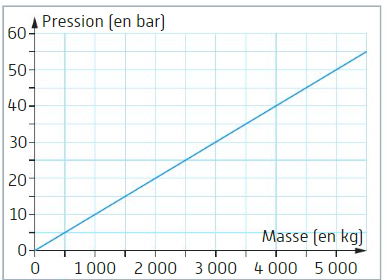
\includegraphics[width=\textwidth]{images/Act2.png}
\end{minipage}%


\end{enumerate}

\vfill 

\end{document}